% Anhang ist manuell erstellt und verwendet nicht das appendix package
\setcounter{section}{0}
\setcounter{subsection}{0}
\renewcommand*\thesection{\Alph{section}}

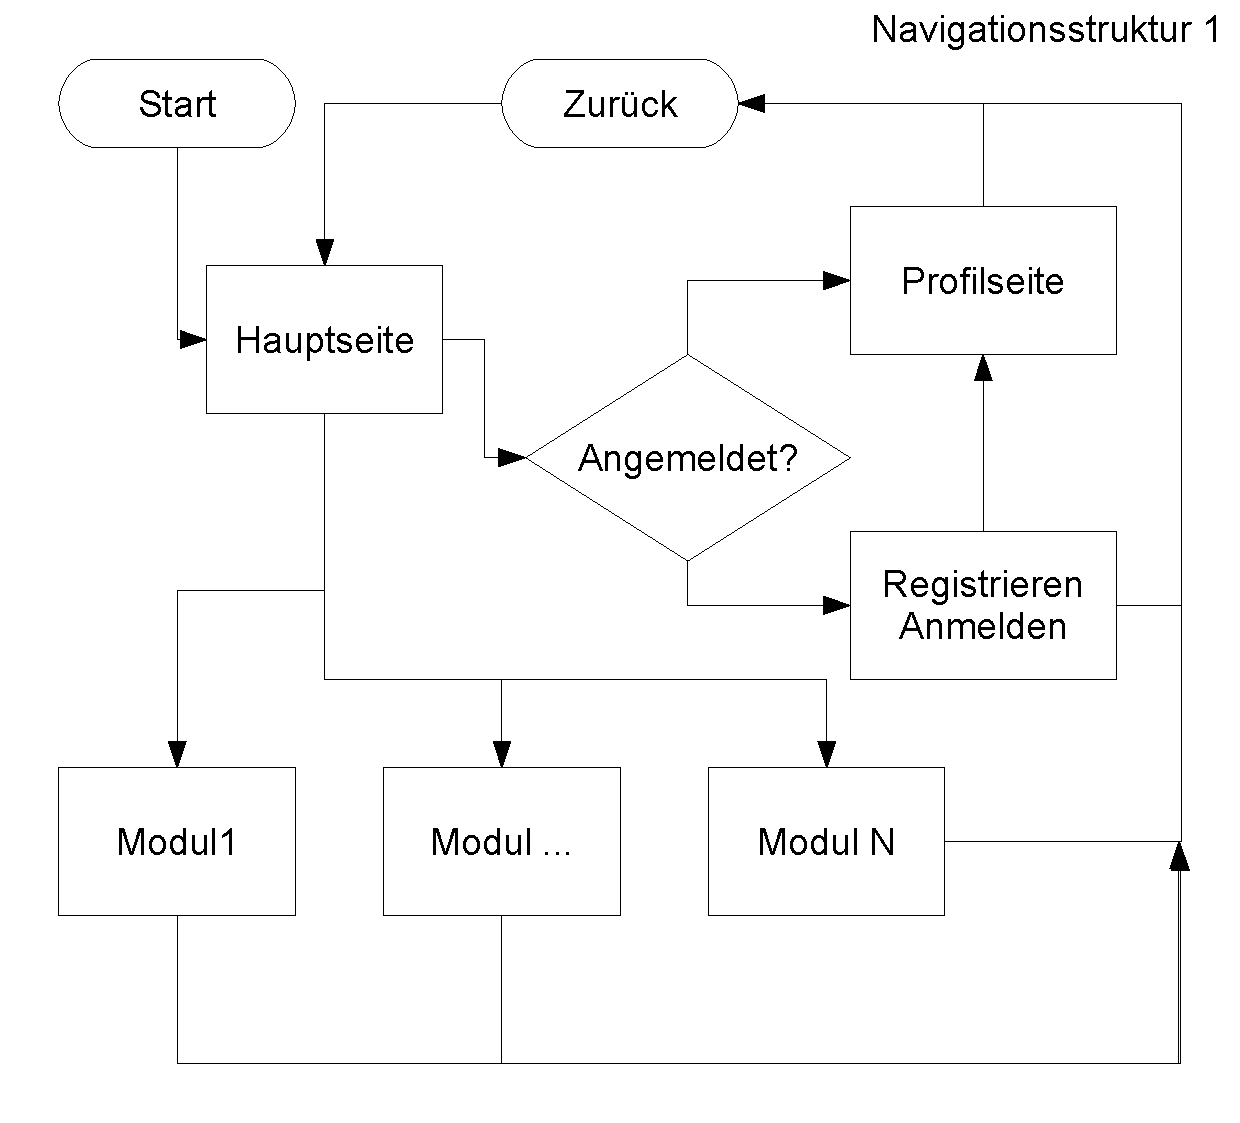
\includepdf[scale=0.8,pages={1},pagecommand=\chapter{Anhang}\section{Navigationsstruktur}\label{fig:nav}]{navigation.pdf}
\includepdf[scale=0.8,pages={2},pagecommand=\section{Navigationsstruktur2}\label{fig:nav2}]{navigation.pdf}

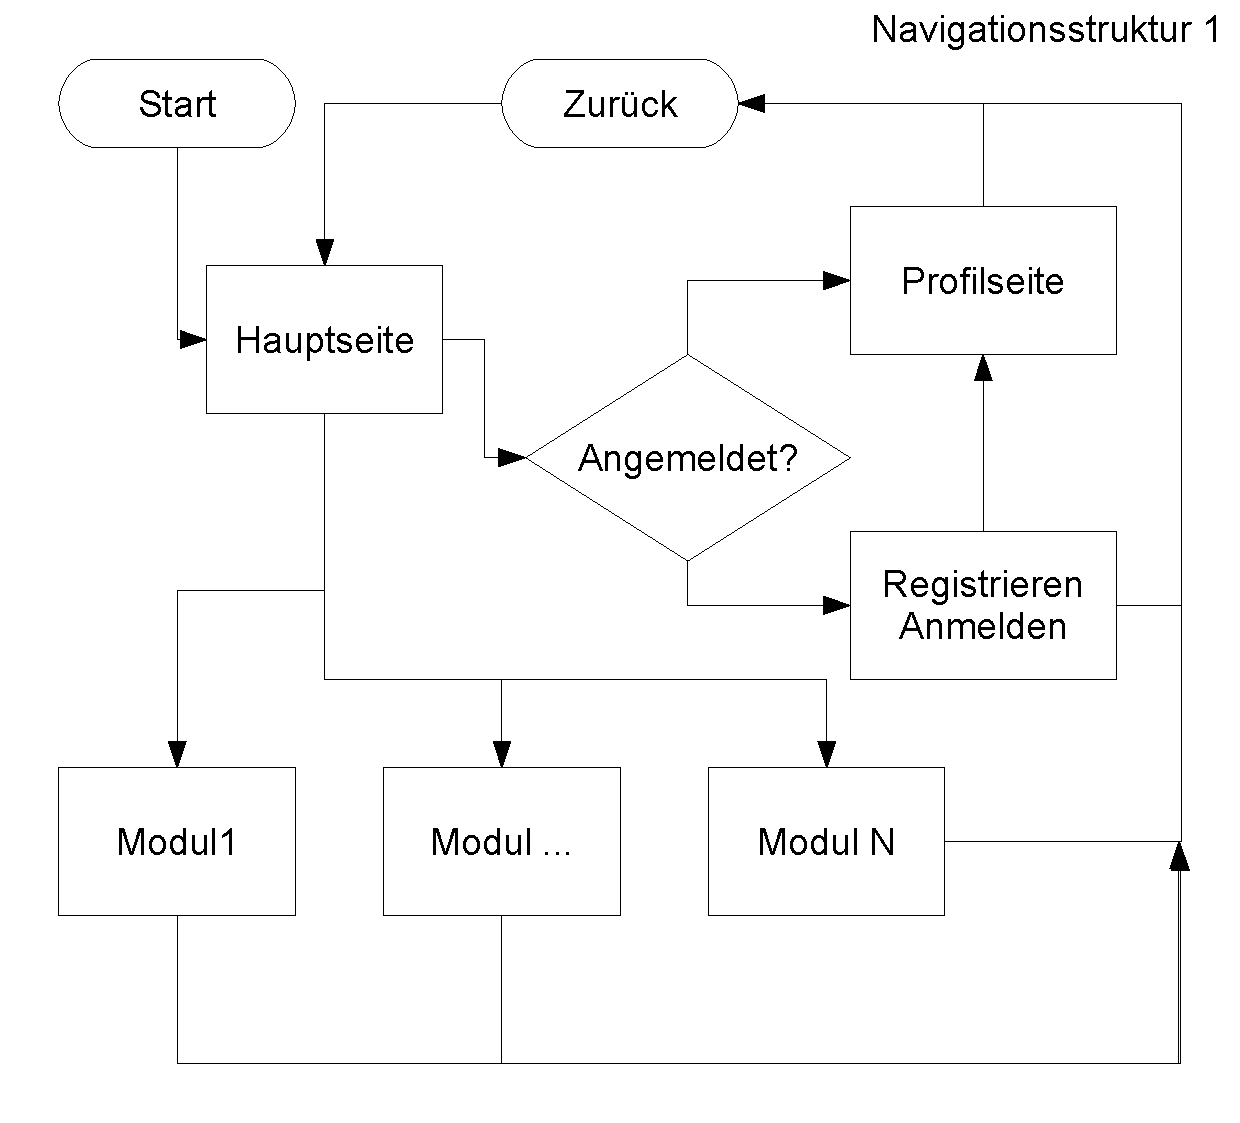
\includepdf[scale=0.8,pages={1},pagecommand=\section{Layout}\label{fig:layout}]{struktur.pdf}
\includepdf[scale=0.8,pages={2-7}]{struktur.pdf}

\subsection{Icons}
\begin{tabular}{ | p{0.42\textwidth} | p{0.55\textwidth} | } 
	\texttt{layout/module-page-icon.png}	& Navigationsicon\\
	\texttt{layout/main-page-icon.png}	& Navigationsicon\\
	\texttt{layout/login-icon.png}	& Navigationsicon\\
	\texttt{layout/profile-icon.png}	& Navigationsicon\\
	\texttt{layout/help-icon.png}	& Navigationsicon\\
	\texttt{layout/learn-icon.png}	& Navigationsicon\\
	\texttt{layout/practise-icon.png}	& Navigationsicon\\
	\texttt{layout/success-icon.png}	& Erfolgsicon\\
	\texttt{layout/fail-icon.png}	& Erfolgsicon\\
\end{tabular}

\subsection{Texte}
\begin{tabular}{ | p{0.42\textwidth} | p{0.55\textwidth} | } 
	\texttt{layout/index.html}	& Inhalt für die Hauptseit\\
\end{tabular}

\section{Modul Vokabeltrainer}
\subsection{Texte}
\begin{tabular}{ | p{0.42\textwidth} | p{0.55\textwidth} | } 
	\texttt{vocabulary/index.html}	& Hauptseite. Intro Vokabeltrainer\\
	\texttt{vocabulary/learn/index.html}	& Lern-Hauptseite. Vorstellung der Inhalte\\
	\texttt{vocabulary/practice/index.html}	& Üben-Hauptseite. Vorstellung der Übungen\\
\end{tabular}


\section{Modul Mathematik}
\subsection{Texte}
\begin{tabular}{ | p{0.42\textwidth} | p{0.55\textwidth} | } 
	\texttt{mathematics/index.html}	& Hauptseite. Intro Vedische Mathematik\\
	\texttt{mathematics/learn/index.html}	& Lern-Hauptseite. Vorstellung der Inhalte\\
	\texttt{mathematics/learn/page1.html}	& Alle von 9, den letzten von 10\\
	\texttt{mathematics/learn/page2.html}	& Vertikal und Kreuzweise\\
	\texttt{mathematics/learn/page2a.html}	& Vertikal und Kreuzweise Für kleine Zahlen\\
	\texttt{mathematics/learn/page2b.html}	& Vertikal und Kreuzweise Für Zahlen nahe 100\\
	\texttt{mathematics/learn/page2c.html}	& Vertikal und Kreuzweise Für Zahlen unter 100\\
	\texttt{mathematics/learn/page2d.html}	& Vertikal und Kreuzweise Für kleine Brüche\\
	\texttt{mathematics/learn/page3.html}	& Um 1 mehr als bei dem davor\\
	\texttt{mathematics/learn/page4.html}	& Multiplikation mit 11\\
	\texttt{mathematics/learn/page5.html}	& Division durch 9\\
	\texttt{mathematics/learn/index.html}	& Trainings- Hauptseite.\\
	\texttt{mathematics/learn/page1.html}	& Vertikal und Kreuzweise\\
	\texttt{mathematics/learn/page2a.html}	& Vertikal und Kreuzweise Für kleine Zahlen\\
	\texttt{mathematics/learn/page2b.html}	& Vertikal und Kreuzweise Für Zahlen nahe 100\\
	\texttt{mathematics/learn/page2c.html}	& Vertikal und Kreuzweise Für Zahlen unter 100\\
	\texttt{mathematics/learn/page2d.html}	& Vertikal und Kreuzweise Für kleine Brüche\\
	\texttt{mathematics/learn/page3.html}	& Um 1 mehr als bei dem davor\\
	\texttt{mathematics/learn/page4.html}	& Multiplikation mit 11\\
	\texttt{mathematics/learn/page5.html}	& Division durch 9\\
\end{tabular}

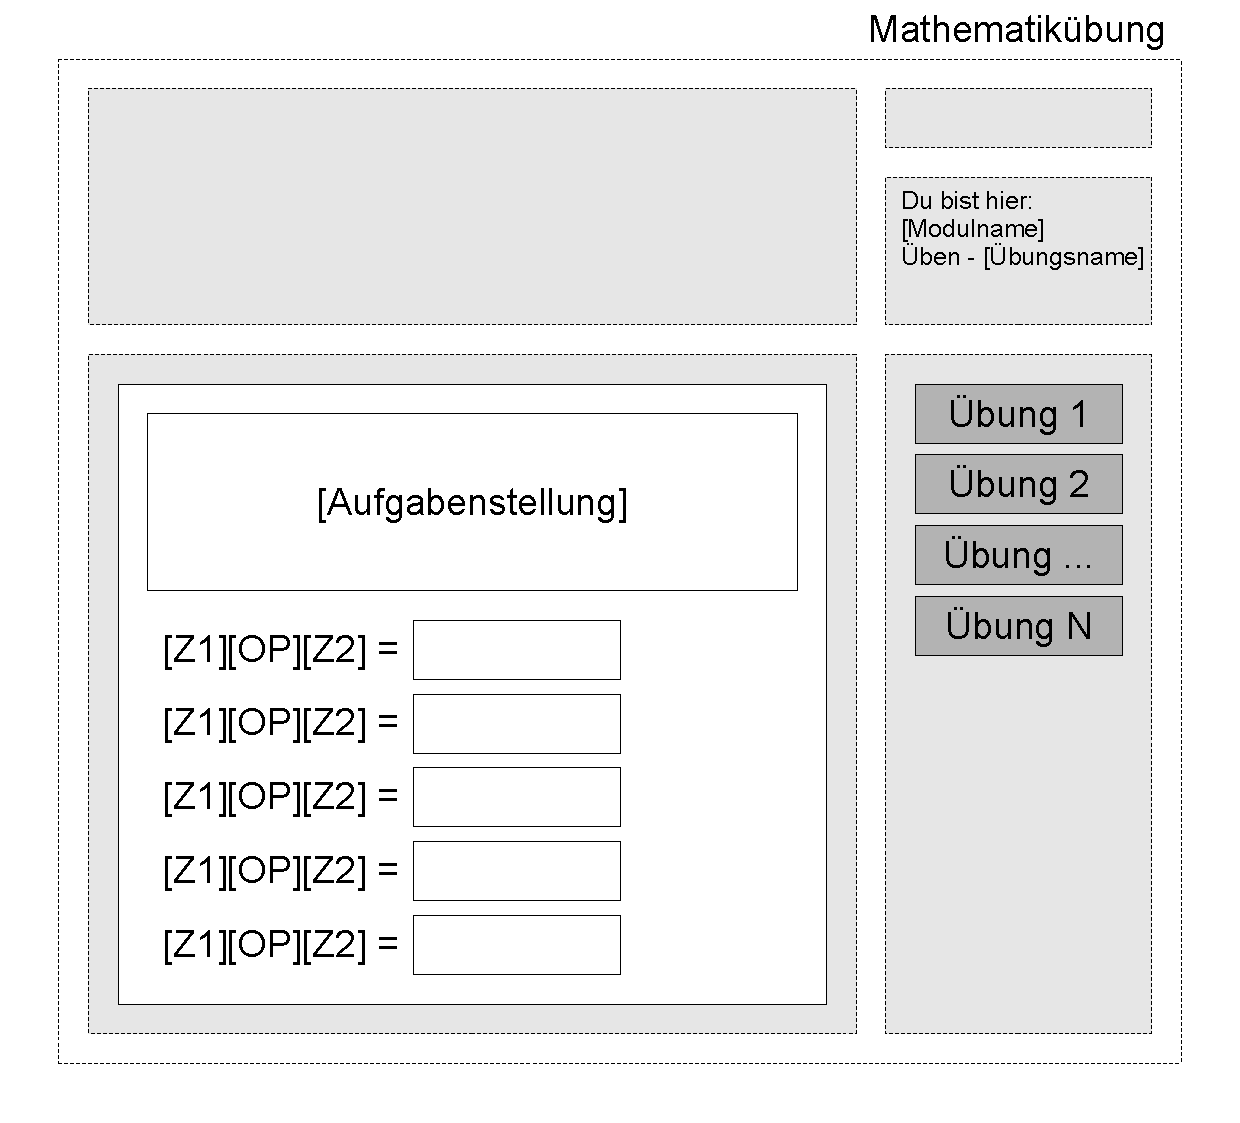
\includepdf[scale=0.8,pages={1},pagecommand=\subsection{Layout}]{math-practise-page.pdf}


